\NeedsTeXFormat{LaTeX2e}[2005/12/01]
%%    2009/03/12 v1.0 GAUBM Vorlage f�r Aschlussarbeiten Physik
%% Template fuer Bachelor- und Masterarbeiten
%% an der Fakultaet fuer Physik (c) Thomas Pruschke der GA Universit�t
%% Verbesserungsvorschlaege bitte an pruschke@theorie.physik.uni-goettingen.de
%%
%% Benoetigte Pakete: datenumber
%%

%%%%%%%%%%%%%%%%%%%%%%%%%%%%%%%%%%%%%%%%%%%%%%%%%%%%%%%%%%%%%%%%%%%%%%
%%%%%%%%%% Bitte vor dem Veraendern diese Datei umbenennen! %%%%%%%%%%
%%%%%%%%%%%%%%%%%%%%%%%%%%%%%%%%%%%%%%%%%%%%%%%%%%%%%%%%%%%%%%%%%%%%%%

%% scrbook - Ersatz f�r LaTeX book Klasse aus dem KOMA Script
%% Moegliche Optionen: diejenigen der Klasse scrbook ausser titlepage

%% deutsche Arbeit:
\documentclass[bachelor,       %% Typ der Arbeit: bachelor oder master
               twoside,        %% zweiseitiges Layout
               BCOR10mm,       %% Bindekorrektur 10 mm
%               liststotoc,nomtotoc,bibtotoc, %% Aufnahme der div. Verzeichnisse
                                              %% ins Inhaltsverzeichnis
               english,ngerman, %% Alternativspr. Englisch, Dokumentspr. Deutsch
%               ngerman,english  %% Alternativspr. Deutsch, Dokumentspr. Englisch
%               final,          %% Endversion; draft fuer schnelles Kompilieren
               ]{GAUBM}

\usepackage{setspace}  %% Zur Setzung des Zeilenabstandes
\usepackage{babel}     %% Sprachen-Unterstuetzung
\usepackage{calc}      %% ermoeglicht Rechnen mit Laengen und Zaehlern
\usepackage[T1]{fontenc}       %% Unterstutzung von Umlauten etc.
\usepackage[utf8x]{inputenc}  %%
%% in aktuellem Linux & MacOS X wird standardmaessig UTF8 kodiert!
%\usepackage[utf8]{inputenc}    %% Wenn latin1 nicht geht ...

\usepackage{amsmath,amssymb} %% zusaetzliche Mathe-Symbole

\usepackage{lmodern} %% type1-taugliche CM-Schrift als Variante zur
                     %% "normalen" EC-Schrift
%% Paket fuer bibtex-Datenbanken
\usepackage[comma,numbers,sort&compress]{natbib}
\bibliographystyle{plainnat}

\newcommand{\tabheadfont}[1]{\textbf{#1}} %% Tabellenkopf in Fett
\usepackage{booktabs}                      %% Befehle fuer besseres Tabellenlayout
\usepackage{longtable}                     %% umbrechbare Tabellen
\usepackage{array}                         %% zusaetzliche Spaltenoptionen

%% umfangreiche Pakete fuer Symbole wie \micro, \ohm, \degree, \celsius etc.
\usepackage{textcomp,gensymb}

%\usepackage{SIunits} %% Korrektes Setzen von Einheiten
\usepackage{units}   %% Variante fuer Einheiten

%% Hyperlinks im Dokument; muss als eines der letzten Pakete geladen werden
\usepackage[pdfstartview=FitH,      % Oeffnen mit fit width
            breaklinks=true,        % Umbrueche in Links, nur bei pdflatex default
            bookmarksopen=true,     % aufgeklappte Bookmarks
            bookmarksnumbered=true  % Kapitelnummerierung in bookmarks
            ]{hyperref}

%% Weiter benoetigte Pakete: datenumber
%% Falls dieses Paket nicht in der Installation vorhanden ist,
%% kann es von der Seite mit diesem Template heruntergeladen werden
%% und in einem LaTeX bekanntem Verzeichnis installiert werden (notfalls
%% dem Verzeichnis mit der Arbeit).
\begin{document}
%%
%%                   Ab hier muessen die Anpassungen geschehen
%%
%% Hier den eigenen Namen einsetzen
\ThesisAuthor{William}{Bode}
%% Hier den Geburtsort einsetzen
\PlaceOfBirth{Helmstedt}
%% Titel Arbeit. Das erste Argument ist der deutsche, das zweite der
%% englische Titel.
\ThesisTitle{Molecular Crowding}{}
%% Erst- und Zweitgutacher/in
%% Ist der/die Betreuer/in nicht identisch mit dem/r Erstgutachter/in,
%% muss diese/r als optionales Argument angegeben werden.
\FirstReferee[Dr.\ \ldots]{Prof.\ Dr.\ Stefan Klumpp}
\Institute{Institut für nichtlineare Dynamik / Theoretische Biophysik}
%\SecondReferee{Prof.\ Dr.\ \dots}
%% Beginn und Ende des Anfertigungszeitraumes
\ThesisBegin{1}{2}{2016}
\ThesisEnd{1}{3}{2016}
%% DO NOT TOUCH THESE LINES!!!!
\frontmatter
\maketitle
\cleardoublepage
%% Zusammenfassung. Falls nicht gewuenscht, bitte auskommentieren.
%%\begin{abstract}
%%  Hier werden auf einer halben Seite die Kernaussagen der Arbeit
%%  zusammengefasst.
%% Optional: Stichwoerter. Wenn nicht gewuenscht, koennen die beiden
%% folgenden Zeilen geloescht werden
%%  \bigskip\par
%%  \textbf{Stichwörter:} Biophysik, Molecular Crowding
%%\end{abstract}
%% So laesst sich in die andere Sprache umschalten (Englisch bzw. Deutsch)
%%\begin{otherlanguage}{english}
%%\begin{abstract}
%%  Here the key results of the thesis can be presented in about
%%  half a page.
%%  \bigskip\par
%%  \textbf{Keywords:} Physics, Bachelor thesis
%%\end{abstract}
%%\end{otherlanguage}

%% Ende des Vorspanns
\cleardoublepage
%% Ab hier 1 1/2 facher Zeilenabstand (durch setspace-Paket)
\onehalfspacing
%% Erzeugt Inhaltsverzeichnis
\tableofcontents

%% Hier kann man seine Bezeichnungsweisen erklaeren. Falls nicht
%% benoetigt, bis einschliesslich \end{nomenclature} auskommentieren
\begin{nomenclature}
%% Fuer die Berechnung der Spaltenbreiten muss \usepackage{calc}
%% geladen sein!
\section*{Lateinische Buchstaben}
\noindent
\begin{longtable}[l]{p{0.2\textwidth}p{0.7\textwidth-6\tabcolsep}p{0.1\textwidth}}
  \tabheadfont{Variable}&\tabheadfont{Bedeutung}&\tabheadfont{Einheit}\\\midrule\endhead
  $A$ & Querschnittsfl"ache & $\unit{m^2}$\\
  $c$ & Geschwindigkeit & $\unitfrac{m}{s}$
\end{longtable}
\section*{Griechische Buchstaben}
\begin{longtable}[l]{p{0.2\textwidth}p{0.7\textwidth-6\tabcolsep}p{0.1\textwidth}}
  \tabheadfont{Variable}&\tabheadfont{Bedeutung}&\tabheadfont{Einheit}\\\midrule\endhead
  $\alpha$  & Winkel & $\unit{\degree}$; --\\
  $\varrho$ & Dichte & $\unitfrac{kg}{m^3}$
\end{longtable}
\section*{Indizes}
\begin{longtable}[l]{p{0.2\textwidth}p{0.8\textwidth-4\tabcolsep}}
  \tabheadfont{Index}&\tabheadfont{Bedeutung}\\\midrule\endhead
  m & Meridian\\
  $r$ & Radial
\end{longtable}
\section*{Abk"urzungen}
\begin{longtable}[l]{p{0.2\textwidth}p{0.8\textwidth-4\tabcolsep}}
  \tabheadfont{Abk"urzung}&\tabheadfont{Bedeutung}\\\midrule\endhead
  2D & zweidimensional\\
  3D & dreidimensional\\
  max & maximal
\end{longtable}
\end{nomenclature}
%% \listoftables und \listoffigures sollten nur bei genuegender Anzahl Tabellen
%% verwendet werden
%\listoffigures
%\listoftables

\mainmatter   %% Anfang Hauptteil

\chapter{Motivation}
Das Innere einer Zelle ist so eng besetzt, dass die mittleren Abstände zwischen
benachbarten Proteinen vergleichbar mit der Größe der Proteine selbst ist.
Daher sind Betrachtungen, die von einer freien Bewegung in einer Zelle ausgehen,
nicht ausreichend für eine korrekte Beschreibung von Diffusionskinetik und Gleichgewichtszuständen.
Daher soll in diesem Spezialisierungspraktikum der Einfluss von \emph{Crowding}
untersucht werden, also dem dichten Besetzen einer Zelle mit Proteinen, die weder
Ligand noch Rezeptor in einer zu betrachtenden Reaktion sind.


\chapter{Grundlagen}
\section{Rezeptor-Ligandenbindung}

Aus dem Massenwirkungsgesetz ist für eine Reaktion zwischen Liganden L und Rezeptoren R der Begriff
der Dissoziationskonstante gegeben:
\begin{equation}
K_d = \frac{[L][R]}{LR}
\end{equation}
Das umschreiben als

\begin{equation}
\label{er}
[LR] = \frac{[L][R]}{K_d}
\end{equation}

Uns werden später die Bindewahrscheinlichkeiten interessieren. Diese sind nun gerade gegeben durch:
\begin{equation}
p_{bound} = \frac{[LR]}{[R]+[LR]}
\end{equation}

Setzen wir nun \ref{er} ein erhalten wir:

\begin{equation}
\label{pbounddiss}
p_{bound} = \frac{[L]/K_d}{1+([L]/K_d)}
\end{equation}



\section{Betrachtung mittels Statistischer Mechanik}
Ein wichtiges Werkzeug zur Betrachtung einer Zelle ist der Formalismus der
Statistischen Mechanik. Die Zelle kann als chemisches oder mechanisches Gleichgewicht
betrachtet werden, in der die niedrige Energiezustände und Entropieerhöhung angestrebt
werden. Das Ziel soll nun sein, eine Boltzmannverteilung herzuleiten, welche die
Wahrscheinlichkeit eines Mikrozustands basierend auf einer Energie beschreibt.
Zunächst wird die Boltzmannverteilung nur für Liganden und Rezeptor hergeleitet,
dann um Crowding erweitert
Die folgenden Berechnungen sind im wesentlichen Kapitel 6 und 14 von
\cite{phybio} nachvollzogen.

\subsection{Partikelarrangements Zählen}

Betrachtet man ein Gitter mit $\Omega$ Plätzen auf dem $L$ Liganden zu verteilen
sind, so gibt es für den ersten Liganden $\Omega$ mögliche Plätze. Danach gibt es
für den nächsten der $L - 1$ möglichen Plätze $\Omega - 1$ mögliche Plätze.
Dieses Argument wiederholt man insgesamt $L$-mal und kommt auf die möglichen Arrangements:

\begin{equation}
\text{Anzahl Arrangements} = \frac{\Omega!}{(\Omega\text{-}L)!}
\end{equation}

In unserem Fall sind die Liganden aber ununterscheidbar. Wenn also 2 Liganden
Plätze tauschen würden, so würde sich daraus kein anderer Zustand ergeben. Um
dieses Überzählen zu verhindern, führt man den \emph{Gibbs-Faktor} $\frac{1}{L!}$
ein:

\begin{equation}
\label{zustaende}
\text{Anzahl Zustände} = \frac{\Omega!}{L!(\Omega\text{-}L)!}
\end{equation}

\subsection{Wahrscheinlichkeit von Mikrozuständen}
Das Grundsätzliche Ziel der statistischen Mechanik ist es, Wahrscheinlichkeitsaussagen
über das Auftreten verschiedener Mikrozustände zu treffen. Der wesentliche Unterschied
zwischen zwei Mikrozuständen ist die Energie $E_i$, wobei $i$ den $i$-ten Mikrozustand
bezeichnet. Aus der Statistischen Mechanik ist nun genau die Wahrscheinlichkeit
bekannt, mit der jeweils ein Mikrozustand auftritt:
\begin{equation}
  \label{eq:boltzmann}
  p(E_i) = \frac{1}{Z} e^{\text{-}E_i\text{/}k_bT}
\end{equation}

Der Faktor $\frac{1}{Z}$ dient der Normierung der Verteilung.
Z ist bekannt als die Zustandssumme. Die Gleichung \ref{eq:boltzmann}
ist bekannt als Boltzmann-Verteilung. Die Normalisierungskonstante $\frac{1}{Z}$
kann durch die Anforderung $ \sum_{i=1}^{N} p(E_i) = 1$ bestimmt werden, was bedeutet:
\begin{equation}
Z = \sum_{i=1}^{N}e^{\text{-}E_i\beta}
\end{equation}

$\beta$ ist hier die inverse Temperatur $\frac{1}{k_bT}$

\subsection{Bindewahrscheinlichkeit}
Diese Werkzeuge können nun angewandt werden, um die Bindewahrscheinlichkeit eines
Liganden an einem Rezeptor zu berechnen.

Hierzu bilden wir das Verhältnis aus dem statistischen Gewicht des gebundenen
Zustands und der Summe der statistischen Gewichte der gebundenen und ungebundenen
Zustände. Das Gewicht des gebundenen Zustands ist
$$e^{\text{-}\beta\varepsilon_b} \cdot \sum_{Lösung}e^{\text{-}\beta(L\text{-}1)\varepsilon_{sol}}$$
Wobei der erste Term den gebundenen Liganden beschreibt und der zweite Term die Summe
über alle ungebundenen Liganden in der Lösung ist. Wir haben hier $\varepsilon_b$ als
die Bindungsenergie und $\varepsilon_{sol}$ als die Energie für ein freies Teilchen
in der Lösung eingeführt. Die Summe über die Lösung ist eine Anweisung dafür,
über alle Konfigurationen von $L-1$ Teilchen auf $\Omega$ Plätzen zu summieren,
wobei jede davon das Gewicht $e^{-\beta(L-1)\varepsilon_{sol}}$ hat.
Da der Boltzmannfaktor für all diese Zustände gleich ist, gilt es nur
die Anzahl an Konfigurationen zu finden, das führt zu:

\begin{equation}
\label{gebundenerligand}
\sum_{Lösung}e^{\text{-}\beta(L\text{-}1)\varepsilon_{sol}} = \frac{\Omega!}{(L-1)![\Omega-(L-1)]!}e^{-\beta(L-1)\varepsilon_{sol}}
\end{equation}

Desweiteren benötigen wir für die weitere Betrachtung die Zustandssumme,
welche eine Summe ist aus den möglichen gebundenen und ungebundenen Zuständen, also:

\begin{equation}
Z(L,\Omega) = \sum_{Lösung}e^{-\beta L\varepsilon_{sol}} + e^{-\beta\varepsilon_b}\sum_{Lösung}e^{-b(L-1)\varepsilon_{sol}}
\end{equation}

Wir haben den zweiten Term schon in \ref{gebundenerligand} bestimmt, daher fehlt noch der erste.
Hierzu kommen wir mit Gleichung \ref{zustaende} auf:

\begin{equation}
\sum_{Lösung}e^{-\beta L\varepsilon_{sol}} = e^{-\beta L\varepsilon_{sol}}\frac{\Omega!}{L!(\Omega\text{-}L)!}
\end{equation}

Somit können wir die Zustandssumme wie folgt ausdrücken:
\begin{equation}
Z(L,\Omega) = e^{-\beta L\varepsilon_{sol}}\frac{\Omega!}{L!(\Omega\text{-}L)}! + e^{-\beta\varepsilon_b}e^{-\beta(L-1)\varepsilon_{sol}} \frac{\Omega!}{(L-1)![\Omega-(L-1)]!}
\end{equation}

Man kann nun folgende Näherung rechtfertigen:\cite{phybio}
\begin{equation}
\frac{\Omega!}{(\Omega-L)!} \approx \Omega^L
\end{equation}

Nun können wir die Bindewahrscheinlichkeit $p_{bound}$ folgendermaßen ausdrücken:
\begin{equation}
p_{bound} = \frac{e^{-\beta\varepsilon_b}\frac{\Omega^{L-1}}{(L-1)!}e^{-\beta(L-1)\varepsilon_{sol}}}{\frac{\Omega^L}{L!}e^{-\beta L\varepsilon_{sol}} + e^{-\beta\varepsilon_b}\frac{\Omega^{L-1}}{(L-1)!}e^{-\beta(L-1)\varepsilon_b}}
\end{equation}
erweitern wir diesen Bruch um $(L!/\Omega^L)e^{\beta L\varepsilon_{sol}}$ und definieren
$\Delta\varepsilon = \varepsilon_b -\varepsilon_{sol}$, so vereinfacht sich der Ausdruck zu:

\begin{equation}
\label{pboundeasy}
p_{bound} = \frac{(L/\Omega)e^{-\beta\Delta\varepsilon}}{1+(L/\Omega)e^{-\beta\Delta\varepsilon}}
\end{equation}
\subsection{Verbindung Stat. Mech und Chemie}
Vergleichen wir Gleichung \ref{pboundeasy} mit Gleichung \ref{pbounddiss} so erhalten wir folgende Identität:
\begin{equation}
\label{mechchem}
K_d = \frac{1}{v}e^{\beta\Delta\varepsilon},
\end{equation}
Wobei $v$ die Größe eines Gitterzellenvolumens darstellt.
Diese Gleichung erlaubt uns die chemische Betrachtung mit der statistischen Mechanik zu verbinden.


\subsection{Crowding}
Das hergeleitete Gittermodell muss nun noch um Crowdermoleküle erweitert werden.
Mit den selben Argumenten wie bei Gleichung \ref{zustaende} kommt man nun für C Crowdermoleküle auf die Zustandssumme
\begin{equation}
Z_{sol}(L,C) = \frac{\Omega!}{L!C!(\Omega-L-C)!}e^{-\beta L\varepsilon_L^{sol}}e^{-\beta C\varepsilon_C^{sol}}
\end{equation}
wobei $\varepsilon_C^{sol}$ und $\varepsilon_L^{sol}$ die Energien von Crowderpartikel und Ligand darstellen.
Der Rezeptor ist nun entweder besetzt oder nicht besetzt, die Gewichte dieser beiden Zustände sind nun
$Z_{sol}(L-1,)e^{-\beta\varepsilon_L^b}$ und $Z_sol(L,C)$. Die Bindewahrscheinlichkeit für ein Partikel ist daher:
\begin{equation}
p_{bound} = \frac{Z_{sol}(L-1,C)e^{-\beta\varepsilon_L^b}}{Z_{sol}(L-1,C)e^{-\beta\varepsilon_L^b}+Z_{sol}(L,C)}
\end{equation}.
Erweitert man den Bruch nun um $Z_{sol}(L-1,C)e^{-\beta\varepsilon_L^b}$ und geht davon aus dass
$\Omega-L-C \gg 1$ gilt, nimmt die Gleichung folgende einfache Form an:
\begin{equation}
p_{bound} = \frac{1}{1+\frac{\Omega-L-C}{L}e^{\beta\Delta\varepsilon_L}}
\end{equation}
wobei wir die Energiedifferenz $\Delta\varepsilon_L = \varepsilon_L^b - \varepsilon_L^{sol}$ definiert haben.

Führt man noch eine Crowderkonzentration $\phi_C = C/\Omega$ ein, gilt desweiteren:

\begin{equation}
p_{bound} = \frac{1}{1+\frac{\Omega}{L}(1-\phi_C)e^{\beta\Delta\varepsilon_L}}
\end{equation}

Im Vergleich mit Gleichung \ref{mechchem} erfahren wir nun, dass für die Dissoziationskonstante unter
Einfluss von Crowdern gilt:
\begin{equation}
K_d{\phi_C} = (1-\phi_C)\cdot K_d(\phi_C = 0)
\end{equation}
Dieser Ausdruck beschreibt den Einfluss von Crowder bezüglich der Bindungswahrscheinlichkeit.



\section{Simulationsmethoden}
Diese Beschreibungen folgen im Wesentlichen den Bedingungen von \cite{frontphy}
\subsection{Random Walk}
Lässt man Bindungen und Wechselwirkungen außen vor, so handelt es sich bei der
Bewegung eines Liganden in einer Zelle um einen \emph{Random Walk}.
Im eindimensionalen Fall wird bei einem Random Walk ein Objekt auf
einen diskreten Zahlenstrahl mit Schrittabstand $l$ gesetzt.
Pro arbiträr definierten Zeitschritt $\tau$ bewegt sich das das Objekt nun mit gleicher Wahrscheinlichkeit
nach Links oder nach Rechts. Auf ein dreidimensionales Gitter verallgemeinert ist die Wahrscheinlichkeit
für jede Richtung (Vorne, Hinten, Oben, Unten, Links, Rechts) $\frac{1}{6}$.
In einem freien Volumen $V = \Omega l^3$ mit Gitterabstand $l$ und $\Omega$ Gitterplätzen
würde sich das Partikel also mit einer Diffusionskonstante $D = l^2 / (6\tau)$ bewegen.
Wenn $P$ Partikel vorliegen, die sich bewegen sollen, so wählen wir $P$ mal zufällig ein Partikel aus,
das sich bewegt, so dass auf Dauer jedes Partikel durchschnittlich einmal pro Zeitschritt bewegt wird.

\subsection{Gittermodell}
Wir betrachten nun ein dreidimensionales Gittervolumen
$V = \Omega l^3$ mit Gitterabstand $l$ und $\Omega$ Gitterplätzen und statten es mit
$R$ Rezeptoren, $L$ Liganden und $C$ Crowdern, alle zufällig platziert aus.
Wir betrachten der Einfachheit halber, dass Rezeptor, Liganden und Crowder alle gleich groß sind.
Wenn auf diesem Gitter Bewegung stattfindet, so gilt ein Volumenausschluss: Ein Gitterplatz kann nur
von einem Partikel besetzt sein, und sollte ein Partikel sich auf einen besetzten Gitterplatz bewegen
"wollen", so passiert nichts. Desweiteren ist es für Crowderpartikel verboten, den Platz am Rezeptor zu
besetzen.
\subsection{Bindung}
Sobald ein Ligand auf einen Rezeptorplatz kommen, soll mit einer Wahrscheinlichkeit von
1 eine Bindung eingegangen werden. Da das System so in einen energetisch niedrigeren
Zustand kommt, ist die Wahrscheinlichkeit dass es sich von diesem Platz löst verringert.
Diese  Wahrscheinlichkeit, in einem Zeitschritt gebunden zu bleiben(im Folgenden: Stickyness), ist nun gerade da Verhältnis aus $\Omega$ und der Dissoziationskonstante ohne Crowdereinfluss:
\begin{equation}
Stickyness = \frac{\Omega}{e^{\beta\Delta\varepsilon_L}}
\end{equation}

\chapter{Programmbeschreibung}
Zur Simulation des in der Theorie beschriebenen Sachverhalts wurde nun ein Computerprogramm geschrieben, das
vereinfacht gesagt folgende Dinge tut:
\begin{itemize}
\item Erstelle ein Dreidimensionales Gitter mit $\Omega = l^3$ Plätzen und periodischen Randbedingungen
\item Besetze dieses Gitter mit $L = \phi_L\Omega$ Liganden und $C = \phi_C\Omega$ Crowdern sowie 1 Rezeptor
\item Gebe eine Stickyness vor
\item Gebe N Zeitschritte vor
\item Bewege N Zeitschritte lang zufällig $(C+L)$ Teilchen unter Beachtung von Volumenausschluss
\item Speichere die Zeiten zu denen ein Ligand gebunden ist
\item Gebe die Bindewahrscheinlichkeit, die mittlere Bindedauer und die mittlere ungebundene Dauer aus
\end{itemize}

\chapter{Ergebnisse}
Besagte Simulation wurde nun einige Zeit lang laufen gelassen.
Abbildung~\ref{fig:ProbGegenCrowder} zeigt den Verlauf der Bindewahrscheinlichkeit
gegen die Crowderkonzentration für ein Gitter mit $\Omega = 8^3$ Plätzen und einer
Stickyness von 500. Angelegt wurde folgender Fit für für $K_d$ :
\begin{equation}
P_b(\phi_C) = \frac{1}{1+(512K_d)(1-\phi_C)}
\end{equation}
Das Ergebnis ist
\begin{equation}
K_d = 0.002033 \pm 0.0000206
\end{equation}
und weicht vom Theoretischen Wert $K_{d_{theoretisch}} = 1/500 $ um 7\% ab.

Abbildung \ref{fig:mean} zeigt die mittlere Zeiten für den gebundenen und ungebundenen
Zustand. Interessant hierbei ist, dass die ungebundene Zustand anscheinend nicht von
der Crowderkonzentration beeinflusst wird. Die gebundene Zeit hingegen schon.
Gefittet wurde die Funktion auf $t(\phi) = \frac{b}{1-x}$ mit $b = 505 \pm 6$.

Dies Ergibt Sinn, da im Falle der kompletten Besetzung des Volumens durch Crowdern der
Ligand ständig gebunden wäre.


\begin{figure}
  \centering
  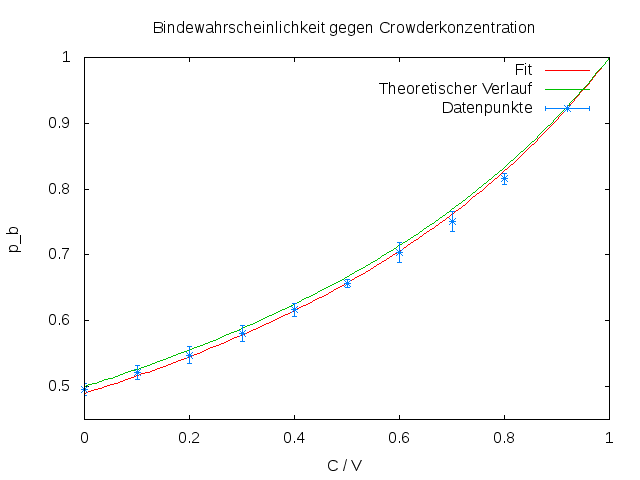
\includegraphics[width=0.9\linewidth]{ProbgegenCrowder.png}
  \caption{Bindewahrscheinlichkeit gegen Crowderkonzentration}
  \label{fig:ProbGegenCrowder}
\end{figure}

\begin{figure}
  \centering
  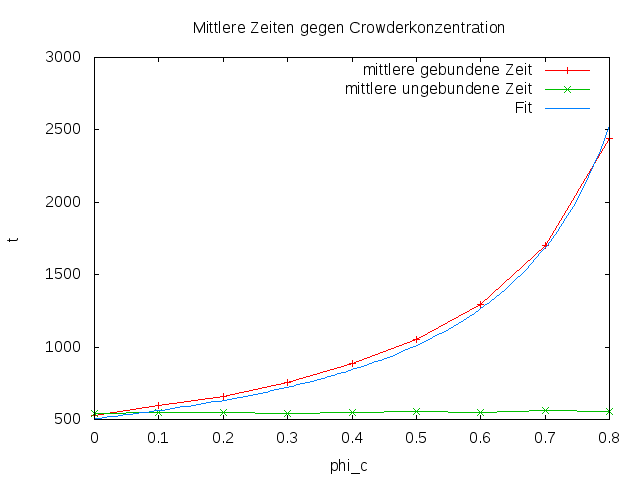
\includegraphics[width=0.9\linewidth]{meantimes.png}
  \caption{Mittlere Zeiten gegen Crowderkonzentration}
  \label{fig:mean}
\end{figure}

%%\appendix
%%\chapter{erster Anhang}
%%\chapter{zweiter Anhang}

\cleardoublepage
%% Bibliographie. Das Argument muss der Name der BIBTeX-Datenbank stehen.
%% Ein Beispiel fuer eine solche Datenbank finden Sie in bthesis_datenbank.bib
\bibliography{bthesis_datenbank}


%% Dieser Befehl MUSS am Ende stehen und erzeugt die Erklaerung ueber die
%% benutzten Mittel
%%\Declaration
\end{document}
